\chapter{Results}

The aim of the methods described in this thesis is to provide tools to query the disequilibrium of sequence evolution. Described in this chapter is the characterisation of the developed methods. I present two new statistics for measuring the magnitude of disequilibrium. I evaluate these statistics on simulated data. I present the application of the test of existence, and test of consistency to simulated data. I complement this with the results of the methods applied to empirical data where I expect disequilibrium to exist.

\section{Methods of Quantifying Disequilibrium}






\section{Is the Human Genome at Equilibrium?}

\begin{figure}[h]
\centering
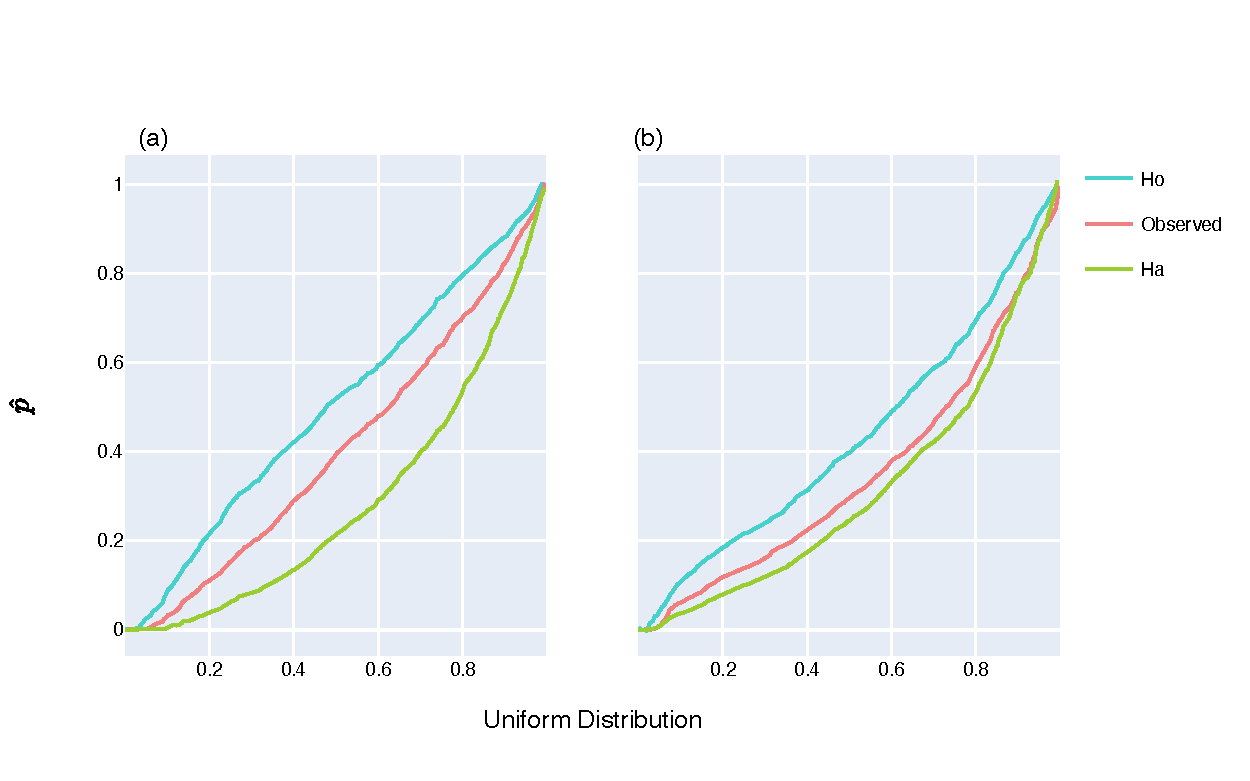
\includegraphics[width=	\textwidth]{figures/plots/primate/LRT-QQ.pdf}
\caption[Humans exhibit a higher proportion of mutation disequilibrium in CDS compared to introns]{\textbf{Humans exhibit a higher proportion of mutation disequilibrium in CDS compared to introns.} The Quantile-Quantile plots compare the distribution of $\hat p-$values to the expected uniform distribution. \textbf{(a)} 1,406 alignments of introns from human, chimpanzee and gorilla, \textbf{(b)}, 1,182 CDS alignments from human, chimpanzee and gorilla. For all model fitting human was the foreground edge. }
\label{fig:primate_lrt_qq}
\end{figure}



The resolution of the LRT $p$ values is too low for conventional methods of multiple test corrections. The simulation results revealed that under the theoretical distribution the $p$ values are not uniformly distributed. As a result, they are unsuitable for assessing significance. A method for assessing significance, in this case, is with a parametric bootstrap. The compute time for a bootstrap with a single replicate is ${\sim} 6$ seconds. For each of the Primate data sets there are ${\sim} 1,300$ alignments. In order to satisfy the Bonferroni correction for $1,300$ alignments you would need to, with some level of precision, be able to estimate $p$ values below the altered significance threshold, $0.05/1,300 = 3.85{\times}10^{-5}$. For it to be possible to reject the null requires generating greater than $3.85{\times}10^{5}$ replicates per alignment. This would take $642$ hours per alignment, of which there are $2,600$. This is a prohibitive level of computation that is both impractical, and unnecessary. 

I have established an alternate strategy that takes advantage of the shape of the distribution. The challenge of correcting for multiple tests is pronounced in the space of genomics, for which \cite{Storey2003StatisticalStudies} introduced a formal procedure for estimating the false discovery rate. In their case, they produce an alternate statistic to be interpreted for an individual result, which isn't applicable here due to the low resolution of $p$ values. However, their procedure included an estimation of the fraction of an analysis which is consistent with the null hypothesis. This method takes advantage of how the $p$ values of data that is consistent with the null will be uniformly distributed, illustrated in Figure 1 of \cite{Storey2003StatisticalStudies}. Fitting a cubic spline to determine the inflection point, one can estimate the proportion of a given distribution that is uniform consistent with the null hypothesis, denoted $\hat \pi_{0}$. Of interest to this analysis is $1 -\hat \pi_{0}$, the proportion that is not consistent with the null hypothesis. The code to produce $\hat \pi_{0}$ is included in the appendices. 

Rates of evolution in introns and exons. If the null was true, and the branch length was the same between introns and exons, then the distribution of the difference would be centered on zero. Try a T-test of the null that the mean is zero, against the prior alternate that the exons are evolving slower, and so the mean is greater than zero. The assumption of the T-test is that the distribution is normal, which is hard to say in this case. The T-test is pretty robust, but I can test for whether it is normally distributed also. 






 
\section{The PAR-half of \textit{Fxy} is further from equilibrium than the non-PAR half in \textit{M. musculus}}